\documentclass{standalone}
\usepackage{tikz}
\usepackage{ctex,siunitx,ninecolors}
\setCJKmainfont{Noto Serif CJK SC}
\usepackage{tkz-euclide}
\usepackage{amsmath}
\usetikzlibrary{patterns, calc}
\usetikzlibrary {decorations.pathmorphing, decorations.pathreplacing, decorations.shapes}
\newcommand{\posthead}[2][gray]{
  \begin{scope}[#2]
    \fill[left color=#1,right color= #1,middle color=#1!20](0,0)ellipse(0.05 and 0.02);
    \fill[left color=#1,right color= #1,middle color=#1!20](0.05,0)rectangle(-0.05,0.07);
    \fill[left color=#1,right color= #1,middle color=#1!20](-0.06,0.07)arc(-180:0:0.06 and 0.02)--(0.06,0.15)--(0.05,0.16)--(-0.05,0.16)--(-0.06,0.15)--cycle;
    \fill[#1!50!gray](0,0.16)ellipse(0.05 and 0.02);
    \foreach \x in {75,45,15,-15,-45,-75}
    {
      \draw[very thin,#1!50!gray]({0.05*sin(\x)},{0.16-0.02*cos(\x)})--({0.06*sin(\x)},{0.15-0.02*cos(\x)})--++(0,-0.08);
    }
  \end{scope}
}
\begin{document}
\small
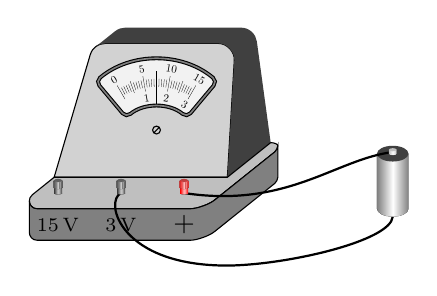
\begin{tikzpicture}[>=latex,scale=1]
  \draw[fill=lightgray!70](-0.842, 1.256)..controls(-0.824, 1.310)and(-0.804, 1.332)..(-0.775, 1.356)..controls(-0.735, 1.387)and(-0.696, 1.399)..(-0.650, 1.400)--( 0.788, 1.400)..controls( 0.894, 1.400)and( 0.994, 1.294)..( 0.988, 1.188)--( 0.900,-0.300)--(-1.300,-0.300)--cycle;
  \draw[double=gray,rounded corners=0.7mm,fill=lightgray!20](130:0.9)--(130:1.2)arc(130:50:1.2)--(50:0.6)arc(50:130:0.6)--cycle;
  \draw[very thin](90:0.63)--(90:1.05);
  \foreach \x in { 60,80,100 }
  {
    \draw[ultra thin](\x:0.8)--++(\x:0.2)(\x+10:0.82)--++(\x+10:0.16);
    \foreach \y in {1,2,3,4,6,7,8,9}
    {
      \draw[ultra thin](\x+2*\y:0.85)--++(\x+2*\y:0.1);
    }
  }
  \draw[ultra thin](120:0.8)--++(120:0.2)node[inner sep=1pt,rotate=30,above]{\scalebox{0.4}{0}};
  
  \node at (60:1.0)[inner sep=1pt,rotate=-30,above]{\scalebox{0.4}{15}};
  \node at (80:1.0)[inner sep=1pt,rotate=-10,above]{\scalebox{0.4}{10}};
  \node at (100:1.0)[inner sep=1pt,rotate=10,above]{\scalebox{0.4}{5}};
  \node at (60:0.8)[inner sep=1pt,rotate=-30,below]{\scalebox{0.4}{3}};
  \node at (80:0.8)[inner sep=1pt,rotate=-10,below]{\scalebox{0.4}{2}};
  \node at (100:0.8)[inner sep=1pt,rotate=10,below]{\scalebox{0.4}{1}};
  \draw(0,0.3)circle(0.05)(0,0.3)--++(45:0.05)(0,0.3)--++(-135:0.05);
  \fill[darkgray](-0.525, 1.556)..controls(-0.485, 1.587)and(-0.446, 1.599)..(-0.400, 1.600)--( 1.076, 1.600)..controls( 1.182, 1.600)and( 1.262, 1.516)..( 1.274, 1.427)--( 1.450, 0.140)--( 0.900,-0.300)--( 0.988, 1.188)..controls( 0.994, 1.294)and( 0.894, 1.400)..( 0.788, 1.400)--(-0.650, 1.400)..controls(-0.696, 1.399)and(-0.735, 1.387)..(-0.775, 1.356)--cycle;
  \draw[fill=lightgray](-1.577,-0.522)..controls(-1.605,-0.546)and(-1.614,-0.572)..(-1.615,-0.600)..controls(-1.615,-0.647)and(-1.581,-0.700)..(-1.515,-0.700)--( 0.425,-0.700)..controls( 0.512,-0.700)and( 0.668,-0.645)..( 0.737,-0.590)--( 1.503, 0.023)..controls( 1.522, 0.038)and( 1.541, 0.077)..( 1.541, 0.101)..controls( 1.541, 0.121)and( 1.495, 0.140)..( 1.450, 0.140)--( 0.900,-0.300)--(-1.300,-0.300)--cycle;
  \draw[fill=gray](-1.615,-1.000)..controls(-1.615,-1.047)and(-1.581,-1.100)..(-1.515,-1.100)--( 0.425,-1.100)..controls( 0.512,-1.100)and( 0.668,-1.045)..( 0.737,-0.990)--( 1.503,-0.377)..controls( 1.522,-0.362)and( 1.541,-0.323)..( 1.541,-0.299)--( 1.541, 0.101)..controls( 1.541, 0.077)and( 1.522, 0.038)..( 1.503, 0.023)--( 0.737,-0.590)..controls( 0.668,-0.645)and( 0.512,-0.700)..( 0.425,-0.700)--(-1.515,-0.700)..controls(-1.581,-0.700)and(-1.615,-0.647)..(-1.615,-0.600)--cycle;
  % \posthead{}
  \node at (-1.25,-0.9){\scriptsize\qty{15}{V}};
  \node at (-0.45,-0.9){\scriptsize\qty{3}{V}};
  \node at (0.35,-0.9){$+$};
  \draw[thick](-0.450,-0.500)..controls(-0.670,-0.602)and(-0.471,-1.431)..( 0.918,-1.421)..controls( 1.677,-1.410)and( 2.977,-1.107)..( 3.000,-0.800);
  % \posthead[red]{xshift=0.35cm,yshift=-0.5cm}
  \posthead[darkgray]{xshift=-0.45cm,yshift=-0.5cm}
  \posthead[darkgray]{xshift=-1.25cm,yshift=-0.5cm}
  \fill[left color=gray, right color=gray,middle color=white](2.8,-0.7)arc(-180:0:0.2 and 0.1)--(3.2,0)--(2.8,0);
  \fill[darkgray](3,0)ellipse(0.2 and 0.1);
  \draw[thick]( 0.350,-0.500)..controls( 1.663,-0.700)and( 2.281,-0.067)..( 3.000, 0.020);
  \posthead[red]{xshift=0.35cm,yshift=-0.5cm}
  \fill[left color=lightgray, right color=lightgray,middle color=white](2.95,0)arc(-180:0:0.05 and 0.02)--(3.05,0.05)--(2.95,0.05);
  \fill[lightgray](3,0.05)ellipse(0.05 and 0.02);
\end{tikzpicture}
\end{document}